\documentclass[a4paper,11pt,oneside]{article}

\usepackage{amsmath,amssymb,epsfig}
\usepackage[T1]{fontenc}
\usepackage{ae,aecompl}
\usepackage{url}
\usepackage{subfigure}
\addtolength{\voffset}{-1cm}
\addtolength{\hoffset}{-1cm}
\setlength{\parindent}{0in}
\addtolength{\textwidth}{1.8cm}
\addtolength{\textheight}{1cm}
\addtolength{\parskip}{.5cm}

% Example definitions.
% --------------------
\def\x{{\mathbf x}}
\def\X{{\mathbf X}}
\def\u{{\mathbf u}}
\def\U{{\mathbf U}}
\def\x{{\mathbf x}}
\def\s{{\mathbf s}}
\def\A{{\mathbf A}}
\def\y{{\mathbf y}}
\def\W{{\mathbf W}}
\def\w{{\mathbf w}}
\def\B{{\mathbf B}}
\def\a{{\mathbf a}}
\def\D{{\mathbf D}}
\def\P{{\mathbf P}}
\def\n{{\mathbf n}}
\def\V{{\mathbf V}}
\def\R{{\mathbf R}}
\def\I{{\mathbf I}}
\def\M{{\mathbf M}}
\def\sech{{\mathrm{sech}}}
\def\L{{\cal L}}
\def\Cum{{\rm{Cum}}}
\def\var{{\rm{var}}}
\def\T{{\mathbf T}}
\def\C{{\mathbf C}}
\def\tf{{\emph{t-f}}}


% Title.
% ------
\title{\large{\textbf{HOMEWORK 4}}}
\author{SGN-1156 Signal Processing Techniques\\
\url{http://www.cs.tut.fi/courses/SGN-1156}\\
Tampere University of Technology\\
Germ\'an G\'omez-Herrero, \url{http://germangh.com}}
\date{Due: December 2, 2009, 10:00 AM}



\begin{document}
\maketitle

\noindent \textbf{Instructions}: Remember to write your name in CAPITAL LETTERS in every page. If you use more than one page you should staple all pages together. You should include in your solutions all relevant intermediate steps. At most you can earn 30 points in this homework. Submit your solutions to mailbox 448 (Tietotalo 4th floor) before the dealine.
\vspace{1cm} 

 

\noindent \textbf{PROBLEM 1 (7 points):} Compute the 4-point DTFs of the two real sequences:

\begin{itemize}
\item[] $x_{1}=\{1,\;4,\; -2,\; 0\}$
\item[] $x_{2}=\{-2,\; 0,\; 1,\; 3\}$
\end{itemize}

\noindent using ONLY a single 4-point DFT. You are not allowed to use MATLAB for this problem (but you may use it to check that your result is correct).

\vspace{1cm} 

\noindent \textbf{PROBLEM 2 (8 points):} Compute the linear convolution of the two sequences:

\begin{itemize}
\item[] $x_{1}=\{1,\; 1,\; 2,\; -1,\; 0,\; 1\}$
\item[] $x_{2}=\{1,\;-2,\; 3,\; 2,\; 1,\; 0\}$
\end{itemize}

\noindent using the formula of the convolution and using the DFT. Check that both methods yield the same result. For the computations using the DFT you can use MATLAB but giving the exact commands that you typed and explaining briefly why. See the help of functions \verb|fft| and \verb|ifft|.

\vspace{1cm}

\noindent \textbf{PROBLEM 3 (15 points):} Consider the system shown in Figure~\ref{fig1}. Assume that the input is bandlimited, $X_a(j\Omega)=0$ for $|\Omega|>2\pi\cdot 1000$.

\begin{itemize}
\item[(a)] What constraints must be placed on $L$, $T_1$, and $T_{2}$ in order for $y_a(t)$ to be equal to $x_a(t)$? Sketch the Fourier transforms of $x_a(t)$, $x(n)$, $y(n)$, and $y_a(t)$.
\item[(b)] If $f_1=f_2=20kHz$ and $L=4$, find an expression for $y_a(t)$ in terms of $x_a(t)$. What is the energy of $y_{a}(t)$ with respect to the energy of $x_{a}(t)$?
\end{itemize}

\begin{figure}[h!]
\centering
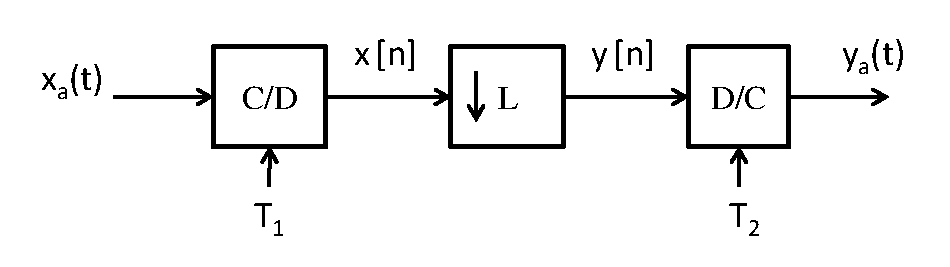
\includegraphics[width=.8\textwidth]{fig1.eps}
\caption{Block diagram of the system of problem 3.}
\label{fig1}
\end{figure} 


\end{document}